\section{Specification- and Syntax-based Linguistic Capability Testing}
\label{sec:approach}

\begin{figure}[thb]
  \centering
  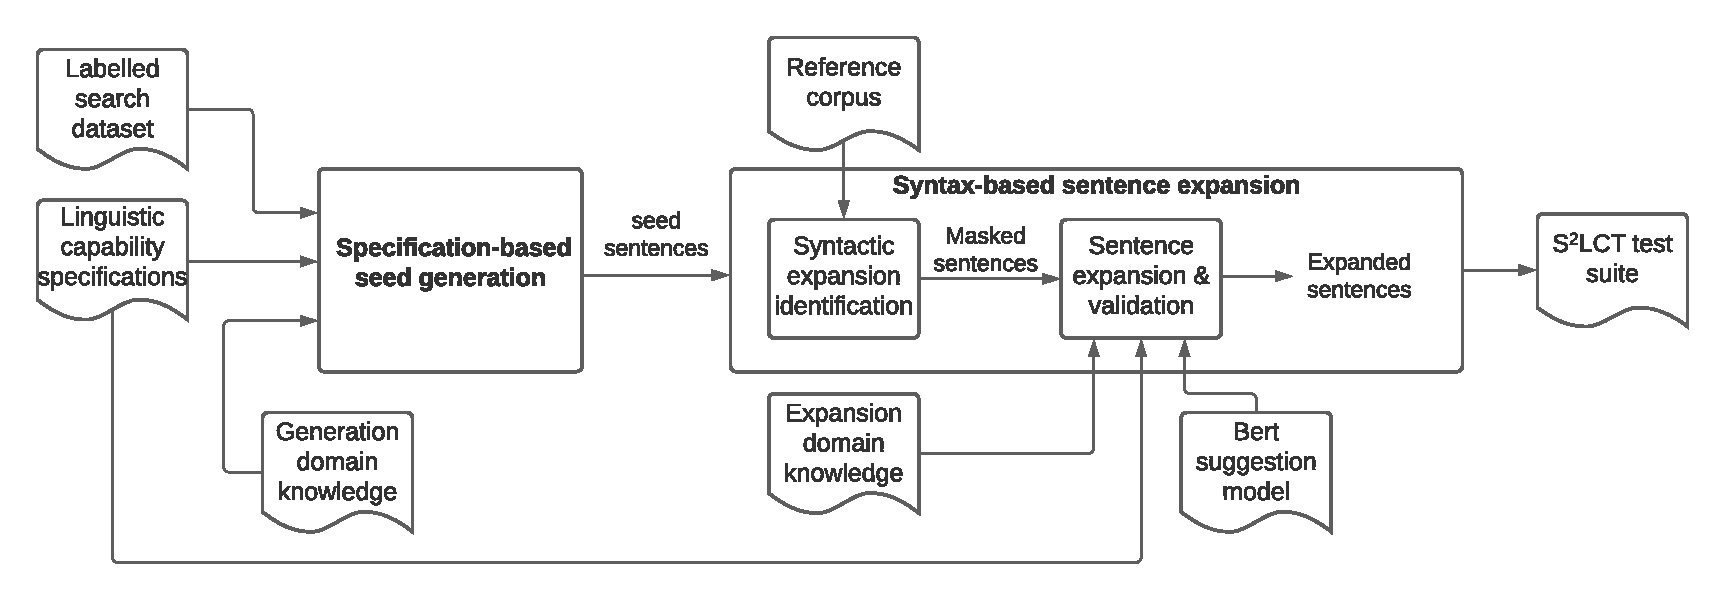
\includegraphics[width=0.49\textwidth]{figs/overview.pdf}
  \vspace{-6mm}
  \caption{\OverviewFigCaption}
\end{figure}

  
  We design and implement a new NLP model testing framework, \tool, which automatically generates test cases with oracles for defined linguistic capabilities to assess the quality of NLP models.

Figure~\ref{fig:overview} depicts an overview of \tool, which
consists of two phases.  The \emph{specification-based seed generation} phase generates the initial set of seed test cases based on generation rules.
Generation rule is consisted of operations and \phs.
\tool provides two built-in operations \texttt{Combine} and \texttt{Replace} and two types of \phs, search-based and enumerative \phs (Section \ref{sec:seed-gen}). 
% The seed generation results in seed test cases that are most likely to conform to a specific \lc and be labelled correctly.
To increase the diversity of test cases generated by \tool, we utilize a \emph{syntax-based sentence expansion} phase (Section \ref{sec:sent-exp}). This phase begins by performing a syntax analysis to identify \pos (PoS) tags that can be added to the seed test cases, by comparing the PoS parse trees of the seed test cases with a large reference corpus of sentences. The identified tags are then inserted into the seed test cases as a \emph{mask}. A masked language model, such as BERT \cite{devlin2019bert}, is then used to suggest words that can fill in the mask. Finally, the resulting sentence is checked to ensure it is consistent with the seed's label and \lc. The generated test suite includes both the original seed test cases and the expanded test cases. This approach enables \tool to cover a wider range of syntactic structures, enhancing its effectiveness in evaluating NLP models.
\vspace{\AlgCompTableVSpace}


% specification which additionally defines the rules for expansion
% (e.g. the expanded word should be \neu).
% Last, because some validated \sents may include
% unacceptable suggested words given the context, we use a heuristic (i.e., the
% confidence score from the NLP recommendation model) to select the more
% realistic context-aware expanded \sents into \tool{}'s test suite.

% We now describe each phase of \tool in detail.

\subsection{Specification-based Seed Generation}
\label{sec:seed-gen}
%\sw{@Jaeseong: I made many changes to this subsection. You need to read through and make sure what I wrote is accurate. @Wei Yang: I think we have been using the terms "seed generation", "\ph", "predicate", and "function" in inconsistent and confusing ways. I think you should take a pass over this subsection to make the presentation accurate.}

%\sw{This may be the general structure we want to discuss our approach in this subsection? (1) We have two seed generation functions: combine and replace. (Describe their high-level functionality.) (2) (Now we describe combine in detail.) Combine has four kinds of parameters, prefix, postfix, infix, and search. (3) Search is a set of sentences from the real-world dataset resulted by applying the predicates: we define two kinds of predicates: implicit and explicit. (4) Prefix, postfix, and infix parameters are sets of user-defined clauses, defined by their relative positions to the search parameter. (5) (Now we describe the replace function). We  implemented negations as an instance of replace function.}

\tool generates the
initial set of seed test cases based on generation rules.
Each generation rule is consisted of operations and \phs.
\tool provides two built-in operations \texttt{combine} and \texttt{replace}.
The \texttt{combine} function takes \phs as parameters, perturbs them in the order as they appear, and returns a collection of seed \sents.
The order of the parameters defines the scope of the \lc.
Specifically,  \tool supports two types of \phs:  enumerative and search-based \phs.
\tool supports four types of \emph{enumerative} \phs, \emph{prefix}, \emph{sent}, \emph{infix} and 
\emph{postfix}.
A \emph{sent} \ph is a collection of the sentences returned by applying the search-based predicates on the real-world dataset (i.e., search-based \phs). 
\emph{prefix}, \emph{infix}, and \emph{postfix} \phs are sets of user-defined clauses, defined by their relative positions to the \emph{sent} \ph.

%\TODO{@Jaeseong, please add description about combine and replace operations}.

% The seed generation phase of \tool takes test cases as the \ph values and 
% performs seed generation on the \phs to match the specifications defined in the \lcs.
% The reasons for this design are twofold.
% First, it generally is infeasible to judge which \lc any \sent falls into and
% which label it should have. 
% Therefore, transforming test cases allows for classifying the resulting test cases
% into individual \lcs with high confidence. This enables us to test each \lc individually. 
% Second, seed generation of test cases from a real-world dataset ensures that our test cases are realistic and diverse. 
% These diverse test cases are more likely to achieve a high coverage of 
% the target model's functionality in each \lc, allowing more comprehensive
% and reliable model evaluation. 
%thus detecting more errors.


% The search-based \ph is a mathematical assertion that verifies 
% a test case in some specific domain of \lc.
In addition to enumerative \phs, \tool also supports search-based \phs. Search-based \phs allow users to define search predicates to construct constraints (in the form of combinational logic) for each linguistic capability.
Search-based \phs enable \tool to find candidate \sents in given 
real-world datasets matching (partial) 
description of each linguistic capability.
%  The search-based \ph is represented as a  of 
% \emph{search predicates}.
\tool supports two types of search predicates as boolean-valued functions, \emph{implicit} and 
\emph{explicit}, which evaluate and verify
that a test case meets the criteria on explicit and implicit linguistic attributes, respectively.
An explicit attribute is an attribute that can be verified directly in the search dataset, while an implicit attribute requires external domain knowledge.
\tool provides a built-in predicate for each type of the attributes (\texttt{hasattr} for explicit attribute and \texttt{contain} for implicit attribute).
% Explicit attribute is different from implicit attribute 
% in that the implicit attribute is not specified explicitly 
% and limited to be verified in test case itself.
%  Accordingly, \emph{hasattr} function
% searches explicit attributes in test case alone while \emph{contain} function explores 
% implicit attributes using external domain knowledge.
% Label attribute is an example of explicit attribute.
For example, for a sentiment analysis, a predicate for any test cases labeled with negative sentiment can be expressed as 
\texttt{hasattr}$(label, negative)$.
For finding test cases with  any neutral adjective words, the predicate can be expressed as $contain(pos, neutral\_adj)$.
The difference between the two cases is that the latter case requires the analysis of each word in the \sent
to identify its semantic and tag of PoS, which may  
not be obtained directly in the search dataset.
Thus, external linguistic  knowledge of tag of PoS and sentiment of word is needed.

\InputWithSpace{tables/lc-requirement-table}
% \InputWithSpace{tables/lc-hsd-requirement-table}

In later phase, after a whole test case is generated, we use combinational logic of 
user-defined predicates to evaluate if the test case is within the scope of a \lc. 
%\sw{I included this example because I think it better illustrates the search-based predicates.}
For example, the second row in Table~\ref{tab:specification} shows the search predicates of the \lc ``\emph{short sentences with sentiment-laden adjectives}". The search predicates define that the sentences with less than 10 tokens (explicit attribute) and have positive/negative labels (explicit attribute) containing positive/negative adjectives or nouns (implicit attributes) are within this linguistic capability.

% In case the search-based \ph only fulfills part of the \lc specifications, 
% we generate seed test cases using \emph{enumerative} \phs.
% The \emph{enumerative} \ph takes the searched \sents, combines them with user-defined
% clauses, and returns seed \sents. We define four types of \emph{enumerative} \phs, \emph{prefix}, \emph{sent}, \emph{infix} and 
% \emph{postfix}, and combine them using a function called \emph{combine} to generate seed test cases.



The third row in Table~\ref{tab:specification} shows an example of the  search-based and enumerative predicates of the \lc ``\emph{negation of negative at the end, should be positive or neutral}'' for \sa. The search-based predicate only finds negative test case using the \emph{hasattr}, expressed as $hasattr(label,negative)$.
In its enumerative predicates, \emph{sent} maps to the searched negative test cases, and \emph{prefix} and \emph{postfix} are user-defined clauses appearing before and after \emph{sent}, respectively.

In addition to the \texttt{combine} operation, \tool also supports \texttt{replace} operations that allow linguistic attributes of \phs be changed in specific ways. 
In this work, we employ negation for some \lcs that requires negation of \sents. Our complete set of seed generation rules is available on the project website.\footnote{\href{https://sites.google.com/view/s2lct/home}{https://sites.google.com/view/s2lct/home}} 
% \sw{This still reads vague. An example of negation could help.}

\paragraph*{Running example.} We use the running example shown in Figure~\ref{fig:ExpEx} to illustrate how \tool works. The first column illustrates the specification-based seed generation phase. Given the \lc ``short sentences with neutral adjectives and nouns'' for the sentiment analysis task, a sentence ``Or both.'' is selected as a seed for the \lc as it satisfies the search-based predicates which require the short sentence be labeled as neutral and has neutral adjective (\ie both). Other sentences in the first column are excluded because their labels are not neutral and/or they include adjectives/nouns that are not neutral, violating the search-based predicates of this linguistic capability.

% (i.e., LC3-LC10 in Table~\ref{tab:specification} and LC11-LC16 and LC19 in Table~\ref{tab:hsd-specification})


% Table~\ref{tab:specification} and~\ref{tab:hsd-specification} shows the search rules and the
% seed generation templates of all 10 linguistic capabilities we
% implemented in \tool for \sa and \hsd tasks respectively. The first column shows the \lc type and its
% description, and the second column shows the search rule and
% seed generation template used in each \lc.

% For LC1 and LC2 in the Table~\ref{tab:specification}, the NLP
% models are evaluated in the scope of short \sents with selective
% sentiment words. It does not require any
% seed generation because the search rules alone are sufficient to find sentences that conform
% to the \lcs. On the other hand, search rules of LC3 to LC10 are not enough to match their \lc specification; thus, \tool additionally uses 
% templates to transform the searched \sents to match the corresponding \lc. For example, in LC3's seed generation template, the searched \sents are appended as part of a sentence to generate a seed.
% In LC4's seed generation template, the searched demonstrative sentences are negated.
% LC1-LC6 in table~\ref{tab:hsd-specification} assess an NLP model on specific semantics expressed in an input sentence such as emotion and threat. Search and seed generation rules are constructed on semantic and structural requirements of test cases described in \lc. Along with it, they are limited to extract inclusive search and seed generation rules that conform to the \lc. In this work, association of search and seed generation rules with the natural language description in \lc is out of our scope, thus we use hatecheck test cases as seed for the \lc, called \textit{hatecheck} in the table.


% \sw{@Jaeseong: revise the rest of 3.1 based on
%   Table~\ref{tab:specification}. I commented out the old text but it
%   is still in the tex file.} \jl{I revised and added the explanation}

%The search phase in \Model searches inputs in dataset and selects
%subset of input \sents in the dataset that meets the \lc
%\req. The idea behind this phase is that input distribution of
%\lc is important to generate inputs relevant to \lc. \Lc explains
%expected behaviors of NLP model on specific types of input and
%output. The NLP model is evaluated on how much it performs on the
%input and output. Thus, \lc introduces the constraints of the input
%data. Input data from the constrained distribution are only qualified
%to be used for evaluating the NLP model on the \lc.  In addition,
%diversity in inputs is important to evaluate NLP models on the
%\lc. Inputs that differ are more likely to cover the NLP model
%behavior, and more coverage increases trustworthiness of the
%evaluation. To generate inputs from same distribution on \lc and high
%diversity of inputs, we estabilish \reqs of input and output
%for each \lc, and find inputs that fulfil the \reqs. Given a
%\lc, a \req consists of search \req, transform
%\req and expansion \req. The search \req
%describes features and functionalities that we seek to have in
%inputs. \Model check each input if it satisfy the \req.

%\begin{figure}[t]
%  \centering
%  \lstinputlisting[language=json-pretty]{code/requirement_sa1.json}
%  \vspace{-10pt}
%  \caption{\SearchRequirementExampleFigCaption}
%  \vspace{-10pt}
%\end{figure}
%
%\begin{figure}[t]
%  \centering
%  \subfloat[][\TransformRequirementExampleSubFigCaption]{\lstinputlisting[language=json-pretty]{code/requirement_sa2.json}}
%  \\
%  \subfloat[][\TransformTemplateExampleSubFigCaption]{\lstinputlisting[language=python]{code/requirement_sa2.py}}
%  \\
%  \caption{\TransformRequirementExampleFigCaption}
%  \vspace{-10pt}
%\end{figure}
%
%Figure~\ref{fig:SearchReqEx} shows \lc of \SareqExOne. To evaluate
%this \lc, the input is required to be short and have only \neu \adjs,
%\neu \nns. In addition, the label needs to be \neu. Therefore, all
%short natural \sents with only \neu \adjs and \neu \nns are available
%to evaluate NLP models. In this work, the sentiment of the words for
%the search are classified based on the sentiment scores from
%\Swn~\cite{baccianella2010sentiwordnet}, a publicly available English
%sentiment lexicons.  It provides lexical sentiment scores and the
%sentiment word labels are categorized by implementing the rules
%in~\cite{mihaela2017sentiwordnetlabel}. Next, transform \req explains
%how the input and output needs to be tranfromed. Some \lc only accepts
%heavily limited input distribution, and it is unlikely to be included
%in searching dataset because of its high structural diversity, thus,
%finding such \sents is costly. Therefore, our approach is to find
%inputs by relaxing search requirement and transform the input to match
%the target requirement of the \lc. In this work, the inputs are
%transformed by word addition or perturbing the found inputs with \lc
%dependent templates. The figure~\ref{fig:TransformReqEx} shows the
%example of use of the template requirement. The \lc of \SareqExTwo in
%the figure~\ref{fig:TransformReqSubEx} requires inputs to be the
%negated \pstv \sents and the \neu expression in the middle. Rather
%than searching \sents that match the input distribution of the \lc,
%the \Model search \pstv and \neu inputs and combine them into negated
%\pstv \sents. Figure~\ref{fig:TransformTempSubEx} illustrates template
%for the \lc. According to the \lc, The value of ``sent1'' and
%``sent2'' become each searched \neu and \pstv inputs respectively, and
%the template completion generates new inputs that matches the target
%\lc. In addition, the seed generation of inputs also produce high
%diversity in the inputs because of that from initially found
%inputs. In this paper, we will denote the searched inputs in this
%phase as seed inputs.

\subsection{Syntax-based \Sent Expansion}
\label{sec:sent-exp}

The seed test cases generated 
may still be limited in their syntactic structures because the search dataset may not cover all the syntax. To address this limitation, we design the syntax-based \sent expansion
phase to extend the seed \sents to cover diverse syntactic structures while still conform to its respective \lc specification.
Our insight is that sentences commonly used in real life cover diverse and realistic syntactic structures that can be used as the basis for the expansion. Thus, in this stage, we differentiate the
parse trees between the seed \sents and a set of reference \sents
obtained from a large real-world dataset. The extra tags of PoS in the reference
parse trees are identified as potential syntactic elements for
expansion and inserted into the seed \sents as masks. We then use
masked language model to suggest the fill-ins. If the resulting
\sents still conform to the \lc specification,
they are added to \tool's test suite.

\subsubsection{Syntax Expansion Identification}

Algorithm~\ref{alg:diff} shows how masks are identified for the seed
\sents.  It takes the parse trees of the seeds, generated by the
Berkeley Neural
Parser~\cite{kitaev2018seedparser,kitaev2019seedparser}, and a
reference context-free grammar (CFG) (i.e., the reference dataset in Figure \ref{fig:overview}) as inputs.
Overall, this algorithm identifies the discrepancy between the seed syntax 
and the reference grammar, which is representative of the distribution of real-world language usage, to decide how a seed and what syntax in the seed can be expanded, producing a set of masked sentences.

\begin{algorithm}
  \caption{\ProdDiffAlgCaption}
  \begin{algorithmic}[1]
    \State \textbf{Input:} Parse trees of seed sentences $\textbf{S}$,
    reference \pcfg$\textbf{R}$
    \State \textbf{Output:} Set of expanded masked sentences $\textbf{S\_exp}$
    \For {$seed$ from $S$}
      \For {each production rule $seed\_prod$ from $seed$}
        \State $seed\_lhs = seed\_prod.lhs$
        \State $seed\_rhs = seed\_prod.rhs$
        \For {$ref\_rhs$, $ref\_prob$ from $R[seed\_lhs]$}
          \If {$seed\_rhs$ is superset of $ref\_rhs$}
            \State $parent = seed\_prod.parent$
            \State $prob = ref\_prob$
            \While {$parent$ is not empty}
              \For {$par\_rhs$, $par\_prob$ from $R[parent.lhs]$}
                \If {$parent.rhs == par\_rhs$}
                  \State $prob = prob \cdot par\_prob$
                  \State $parent = parent.parent$
                  \State break
                \EndIf
              \EndFor  
            \EndWhile
            \State $P.add([seed\_prod, ref\_prod, prob])$
          \EndIf
        \EndFor
      \EndFor
      \If {$P$ is not empty}  
        \State Select Top-k $ref\_prod$ along with probabilities in P
        \For {each $seed\_prod$, $ref\_prod$ in the Top-k selected P}
          \State replace $seed\_prod$ with $ref\_prod$ in $seed$
          \State replace expanded component in $ref\_prod$ with $MASK$
          token in $seed$ sentence
          \State $S\_exp.add([ref\_prod, expanded sentence])$
        \EndFor
      \EndIf
    \EndFor
  \end{algorithmic}
\end{algorithm}


For each production in each seed's parse tree (lines 3 and 4), we
extract its non-terminal at the left-hand-side (line 5), $s\_lhs$, and
the grammar symbols at the right-hand-side (line 6), $s\_rhs$. In line
7, the algorithm iterates through all productions in the reference
CFG and matches these that have the same non-terminal
at the left-hand-side as $s\_lhs$.  The right-hand-side of each
matched production is called $r\_rhs$.  If $s\_rhs$ consists of a
subset of the grammar symbols in $r\_rhs$ (line 8), the additional
symbols in the $r\_rhs$ are inserted as masks in the parse tree of
the seed \sent, in their respective positions in the expanded production.
The left to right traversal of the leaves of an expanded parse tree
forms a masked \sent.
All the masked \sents of each seed are returned at line 14.
% The
% random sampling is unbiased approach since it gives same chance to be
% chosen. Thus, the random sample becomes representative of the
% population of the masked \sents, and it efficiently shows the
% usefulness of the \tool.

\begin{figure*}[t]
  \centering
  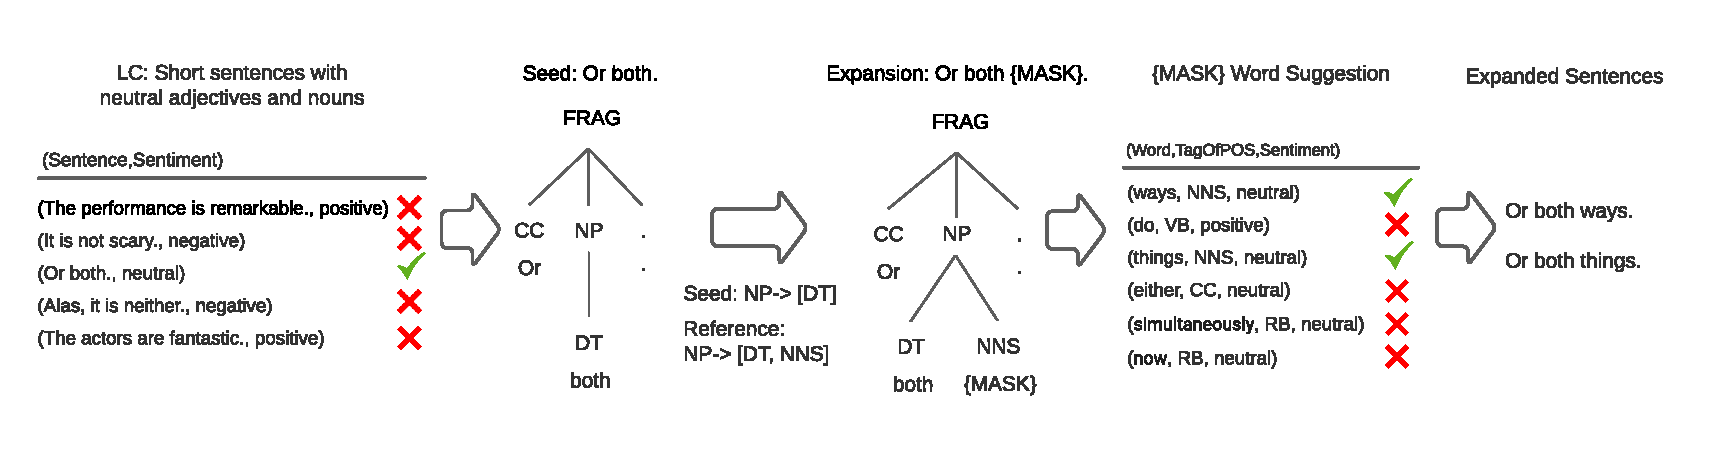
\includegraphics[scale=0.5]{figs/running_example.pdf}
  \vspace{-8mm}
  \caption{Running example of \tool.}
  \label{fig:ExpEx}
\end{figure*}

\paragraph*{Running example.} The second and third columns in Figure~\ref{fig:ExpEx} illustrate how Algorithm \ref{alg:diff} is used to generate a masked \sent. The second column shows the parse tree of the seed \sent ``Or both.", which consists of two productions: $``FRAG\rightarrow[CC, NP, .]"$ and $``NP\rightarrow[DT]"$.
When matching the left-hand-side non-terminal of the second production
(\ie, $``NP"$) in the reference CFG, we found that the reference CFG includes a
production $``NP\rightarrow[DT, NNS]"$ which has an additional symbol ``NNS" on
the right-hand-side. The algorithm thus expands the parse tree with
this symbol, shown in the third column.  The masked \sent ``Or both
\{\emph{MASK}\}." is the result of the left-to-right traversal of this leaves of the
expanded parse tree.

\subsubsection{\Sent Expansion and Validation}
\label{sec:approach:syntaxexpnvalidation}
To expand a masked sentence, the words to fill in the masks are
suggested by the BERT model~\cite{devlin2019bert}.
BERT is a transformer-based \nl model that is pre-trained on masked token prediction task. BERT model is capable of suggesting words for the masked
token according to its surrounding context in a \sent. For each masked
token, multiple words may be suggested, ranked by their confidence scores.
Because BERT model is not aware of the \lc
specification and the grammar symbol in the expanded parse tree, an
expanded \sent using all suggested words may no longer satisfy the
\lc specification or the expanded grammar symbol. Therefore, we perform \emph{validation}
on the suggested words and only accept them if the following three
criteria are met.

First, the tag of PoS of the suggested word must match the PoS tag of the
expanded symbol in the parse tree. For the example in
Figure~\ref{fig:ExpEx}, the masked symbol is a $``NNS"$ (\ie, plural
noun); thus, the suggested word must also be a $``NNS"$. In our implementation, we use the \spacy \cite{spacy} library to extract the tag of PoS for each suggested word.

Second, we require the suggested words be \neu. 
% The sentiment of the expanded \sent must be the same as the seed \sent. However
In general, changing even just one word 
may change the overall label and/or linguistic capability of a \sent, which violates the goal of \tool. To reduce this risk, we only accept neutral words from the suggested words, which requires us to use the expansion domain knowledge to verify the sentiment of each suggested word.

Third, we verify that the expanded \sents satisfy the same \lc specification as their seed
\sents. 
% \sw{Update the following based on what we update in Section 3.1. Currently, the description seems 
% inaccurate and unprincipled.} 
An expanded \sent may no longer be within the scope of its seed's linguistic capability. For example, the predicate shown in the second row of Table \ref{tab:specification}, \emph{\textbf{hasattr}(length,<10)}, may no longer hold after expanding a seed sentence with multiple words.
We only accept an expanded sentence if the search-based predicates are still satisfied and the expansion does not happen within an enuramerate \ph.

% Accordingly, we validate if the expanded \sents are still in the scope of their \lc. 
% Not only that, this criteria may not be applied to other \lcs because enumerative \phs can be used for seed test case generation. In this case, the user-defined enumerative \ph values (e.g. \emph{prefix}, \emph{infix} and \emph{postfix}), are to shift sentiment within the scope of their \lc. Expansion of the \ph values may change context the \ph and fail to conform to the \lc. Therefore, we exclude expansions of syntactic elements within the user-defined \ph values to 
% ensure the expanded \sents within the scope of their \lc.

% In this work, out of the BERT suggested words, we randomly selects
% words that matches their PoS tag of the expanded symbol in the parse
% tree. The words that meets the second and third criteria are finally
% employed for the expanded \sents.

% Our goal for generating the expanded \sents is to use them for
% evaluating the \sa models on the associated \lc in addition to the
% seed \sent. It is only achieved when the expanded \sents are also met
% with the same search rules for the \lc. For LC1 as an example, the
% expanded \sent must still conform to the specification of the seed's
% \lc specification. Therefore, the expanded \sents are required to be
% short and to only have \neu adjectives and \nns.
% \sw{Say why we use
%   the third criteria only for LC1 and LC2.}  \jl{I added the
%   explanation}

\paragraph*{Running example.} The fourth column in Figure~\ref{fig:ExpEx} shows the words suggested by BERT. For this masked \sent, BERT suggested six words. Each word is associated with the tag of PoS and the sentiment. Among the six words, only ``ways'' and ``things'' are validated by \tool because they have the tag of Pos ``NNS'' and are \neu. In addition, both \sents still meet the satisfy the search-based predicates of the \lc \SareqExOne. In the end,  the syntax-based sentence expansion results in two more test cases,  ``Or both ways.'' and ``Or both things.'', from the seed ``Or both.".

%The suggested word are
%validated by three criteria. First, The tag of POS must be matched with
%that suggested from the production differentiation phase. In the
%example in the Figure~\ref{fig:ExpEx}, the mask token comes from the
%structural component of NNS, plural noun. Therefore, the BERT
%suggested words must be also tagged with the NNS. Accordingly, every
%words of the NNS are only available. Second, \Model focuses on the \sa
%task, and it assume that the suggested words must not change sentiment
%of its input and must preserve its consistency of original sentiment
%label. Therefore, we only accept the \neu words for the
%expansion. Third, the expanded \sents with the BERT suggested words
%must be appropriate for evaluating NLP models on the target \lc, and the
%\sents must pass the \req of the \lc. In this work, the BERT
%suggestions are validated by the three criteria.

% \subsubsection{\Sent Selection}
% \sw{@Jaeseong: Add how we select expanded \sents and motivate why.}

% \paragraph{Running example.} \jl{I dont think we need this
%   subsection of \sent selection it is already explained at the
%   previous stage with running example.} \sw{This is to use the bert score to rank and select. Did we discuss this already?}
